\section{Zielsetzung}

In dem Versuch V601 wird die Elektronenhülle eines Quecksilberatomes ($\ce{Hg}$)
untersucht. Das zugrunde liegende Ziel besteht aus der Überprüfung der Bohrschen
Postulate, die 1913 von Nils Bohr formuliert wurden.

\subsection{Hintergrund}

Der Franck-Hertz Versuch beschäftigt sich mit der Quantennatur der
Elektronenhülle eines Atomes. Dieser Versuch
ist nach den Physikern James Franck und Gustav Hertz benannt, die diesen
in den Jahren 1911-1914 ausarbeiteten und durchführten.

\section{Theorie}

Die Elektronenhülle lässt sich über Stoßexperimente erforschen. In dem
Franck-Hertz Versuch werden möglichst monoenergetische Elektronen
auf ein Quecksilbergas geschossen, sodass sie elastisch und unelastisch
mit den Atomgas stoßen.
Im Folgendem wird zuerst der schmatische Aufbau des Versuches dargestellt, da sich anhand
diesem die Gedankenzüge der Theorie verständlicher erläutern lassen.

\subsection{Schematischer Aufbau}

\begin{figure}
  \centering
  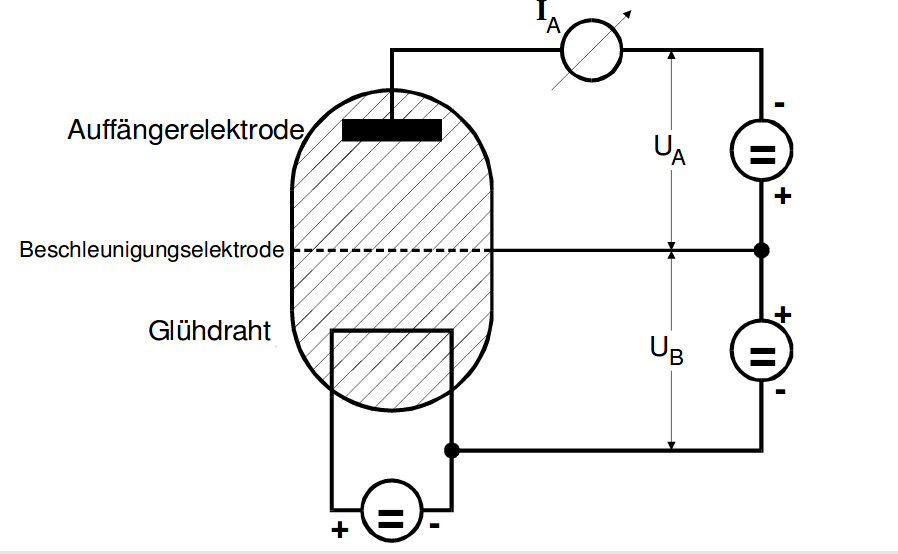
\includegraphics[width=9cm, height=6cm]{Pics/schematisch_Franck_Hertz.png}
  \caption{Schematischer Aufbau des Franck-Hertz Versuches.\cite{anleitung01}}
  \label{fig:schmeatisch_Franck_Hertz}
\end{figure}

Der schematische Aufbau ist in Abb. \ref{fig:schematisch_Franck_Hertz}
dargestellt.
Der schraffierte Bereich im Inneren des Gefäßes ist ein evakuierter Bereich, in dem sich
das $\ce{Hg}-$Gas befindet. Der Glühdraht stellt die Elektronenquelle für
die stoßenden Elektronen dar. Diese liegen aufgrund des Glühelektrischen-Effektes
als Elektronengas um den Glühdrah. Der Glühdraht dient als Kathode.
Die Beschleunigungselektrode ein von der Glühkathode verschiedenes Potential,
welches auf die Elektronen eine anziehende Kraft ausübt. Der Beschleunigungsdraht
dient somit als Anode. Zwischen den beiden erwähnten Elektroden liegt die
Spannung $\su{U}\ua{B}$ an.
Beschleunigte Elektronen nehmen auf der Beschleunigungsstrecke die Energie
$e_0 \cdot\su{U}\ua{B}$ in Form von kinetischer Energie auf.

Die beschleunigten Elektronen landen letztendlich auf der Auffängerelektrode.
Diese besitzt eine Bremsspannung $\su{U}\ua{A}$.
Nur Elektronen, die ausreichend kinietische Energie haben können dieses
Gegenfeld überwinden und an der Auffängerelektrode den Auffängerstrom $\su{I}\ua{A}$
verursachen. Dabei gilt die folgenden Energierelation.

\begin{equation}
  \label{eqn:Überwindungsenergie}
  \frac{m_0}{2}v_z^2 \geq e_0 \su{U}\ua{A}
\end{equation}

Die Elementarladung ist mit $e_0$ zu identifizieren.
Elektronen, die \eqref{eqn:Überwindungsenergie} erfüllen tragen zu
$\su{I}\ua{A}$ bei.

Der Energieverlust der Elektronen durch die Stöße wird mithilfe der Gegenfeldmessung
bestimmt. Das Gegenfeld ist in dem Aufbau \ref{fig:schematisch_Franck_Hertz}
durch die Bremsspannung $\su{U}\ua{A}$ realisiert.
Die Differenz zwischen Anfangsenergie und Endenergie spiegelt die
vom $\ce{Hg}$ aufgenommene Energie wieder.

Bohr postulierte, dass Elektronen nur auf diekreten Bahnen um den Atomkern bewege können.
Für den Franck-Hertz Versuch bedeutet dies, dass der Auffängerstrom
$\su{I}\ua{A}$ bei bestimmten Beschleunigungsspannungen abrupt abfällt.
Diese Energie ist genau dann erreicht, wenn die stoßenden Elektronen
die Quecksilberatome anregen. Der Ablauf ist schematisch wie folgt zu verstehen.

\begin{equation}
  \label{eqn:Reaktionsgleichung}
  \ce{\left(e^-\right)^* + Hg -> Hg^* + e^- -> Hg + \gamma + e^-}
\end{equation}

Dabei makiert $*$ die höher energetischen Zustände.
$\ce{Hg^*}$ ist dabei der erste angeregte Zustand von Quecksilber.
Im ersten angeregten Zustand hat es eine Energie von $\su{E}_1$.
Nach dem angeregeten Zustand geht das $\ce{Hg^*}-$Atom nach einer
Relaxationszeit in der Größenordnung von $\SI{10e-8}{\second}$
unter Aussendung eines $\gamma-$Quantes in den Grundzustand über.
Im Grundzustand hat das Quecksilberatom eine Energie von $\su{E}_0$.
Der Lichtquant $\gamma$ hat eine Energie von

\begin{equation}
  \label{eqn:Lichtquant}
  h\nu = \su{E}_1 - \su{E}_0.
\end{equation}

$h$ ist das Planksche Wirkungsquantum und $\nu$ die Freqeunz des emitierten Lichtes.

Wird die Beschleunigungsspanung dem Auffängerstrom gegenüber aufgetragen
ergibt sich theoretisch die Kurve aus Abb. \ref{fig:Franck-Hertz-Kurve}.

\begin{figure}
  \centering
  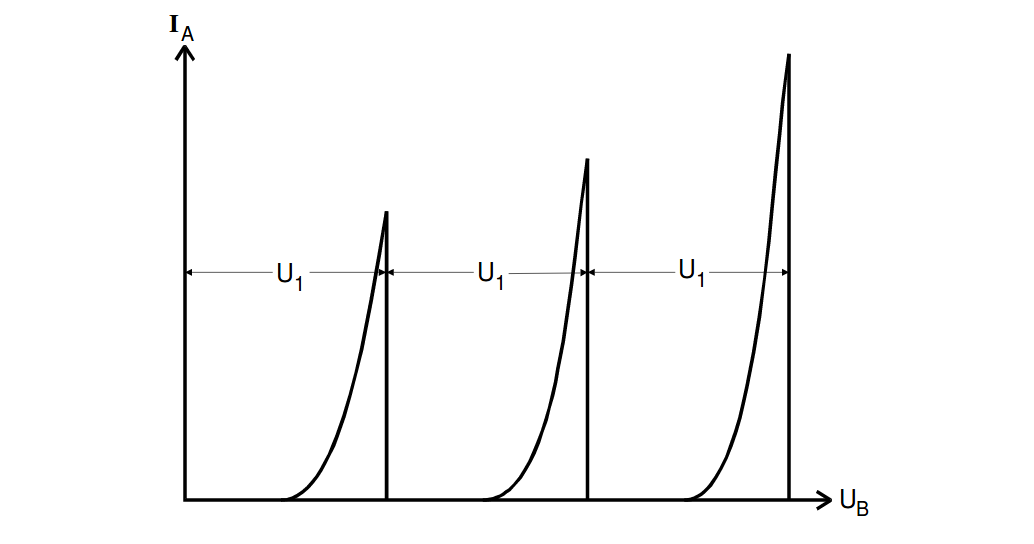
\includegraphics[width=9cm, height=6cm]{Pics/Franck_Hertz_Kurve.png}
  \caption{Theoretische Franck-Hertz-Kurve.\cite{anleitung01}}
  \label{fig:Franck-Hertz-Kurve}
\end{figure}

In den Bereichen in denen kein Auffängerstrom gemessen wird ist die
Energie der Elektronen nicht groß genug, um das Gegenfeld zu überwinden.
Mit steigender Beschleunigungsspannung werden mehr Elektronen von
dem Glühdraht angezogen. Deshalb nehmen die Maxima mit zunehmendem $\su{U}\ua{B}$
ebenfalls zu. Zudem sind die Maxima äquidistant auf der x-Achse angeordnet.
Die Abstände sind gleich dem ersten Anregungspotentials

\begin{equation}
  \label{eqn:Anregungspotential}
  \su{U}_1 = \frac{\left\su{E}_1 - \su{E}_0\right)}{e_0}.
\end{equation}

Abbildung \ref{fig_Franck-Hertz-Kurve} stellt die idealisierte Franck-Hertz-Kurve dar.
